\begin{figure}[htbp!]
    \centering
    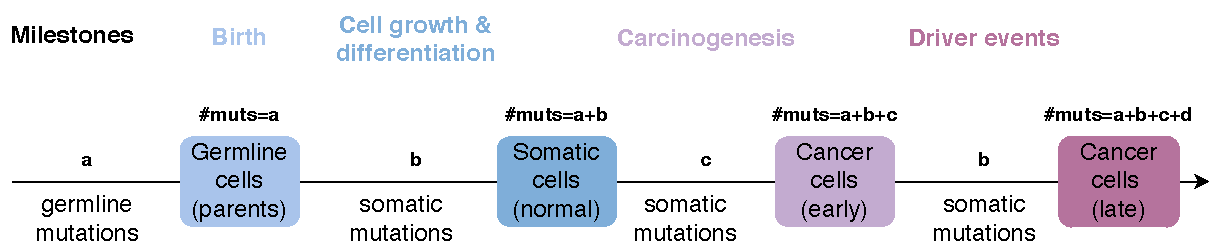
\includegraphics[scale=0.78]{graphics/drivers_demo.pdf}
    \caption{\textbf{Timeline of a carcinogenesis process.} Mutations are almost always retained in the genome after each stage of carcinogenesis (\#muts means the number of mutations). Together, all mutations in a cancer cell make up its mutation profile. For the purpose of this project, only somatic mutations were considered.}
    \label{fig:drivers_demo}
\end{figure}

% \textbf{Timeline of a carcinogenesis process.} Mutations are generally retained in the genome after each stage of carcinogenesis, even though carcinogenesis and driver events could change the phenotype of the cells, (\#muts means the number of mutations). Together, all mutations available in a cancer cell make up its mutation profile. For the purpose of this project, only somatic mutations are considered because germline mutations are not the product of the environment of the differentiated cells in which cancer develops.